\documentclass[11pt]{article}\usepackage[]{graphicx}\usepackage[]{color}
%% maxwidth is the original width if it is less than linewidth
%% otherwise use linewidth (to make sure the graphics do not exceed the margin)
\makeatletter
\def\maxwidth{ %
  \ifdim\Gin@nat@width>\linewidth
    \linewidth
  \else
    \Gin@nat@width
  \fi
}
\makeatother

\definecolor{fgcolor}{rgb}{0.345, 0.345, 0.345}
\newcommand{\hlnum}[1]{\textcolor[rgb]{0.686,0.059,0.569}{#1}}%
\newcommand{\hlstr}[1]{\textcolor[rgb]{0.192,0.494,0.8}{#1}}%
\newcommand{\hlcom}[1]{\textcolor[rgb]{0.678,0.584,0.686}{\textit{#1}}}%
\newcommand{\hlopt}[1]{\textcolor[rgb]{0,0,0}{#1}}%
\newcommand{\hlstd}[1]{\textcolor[rgb]{0.345,0.345,0.345}{#1}}%
\newcommand{\hlkwa}[1]{\textcolor[rgb]{0.161,0.373,0.58}{\textbf{#1}}}%
\newcommand{\hlkwb}[1]{\textcolor[rgb]{0.69,0.353,0.396}{#1}}%
\newcommand{\hlkwc}[1]{\textcolor[rgb]{0.333,0.667,0.333}{#1}}%
\newcommand{\hlkwd}[1]{\textcolor[rgb]{0.737,0.353,0.396}{\textbf{#1}}}%

\usepackage{framed}
\makeatletter
\newenvironment{kframe}{%
 \def\at@end@of@kframe{}%
 \ifinner\ifhmode%
  \def\at@end@of@kframe{\end{minipage}}%
  \begin{minipage}{\columnwidth}%
 \fi\fi%
 \def\FrameCommand##1{\hskip\@totalleftmargin \hskip-\fboxsep
 \colorbox{shadecolor}{##1}\hskip-\fboxsep
     % There is no \\@totalrightmargin, so:
     \hskip-\linewidth \hskip-\@totalleftmargin \hskip\columnwidth}%
 \MakeFramed {\advance\hsize-\width
   \@totalleftmargin\z@ \linewidth\hsize
   \@setminipage}}%
 {\par\unskip\endMakeFramed%
 \at@end@of@kframe}
\makeatother

\definecolor{shadecolor}{rgb}{.97, .97, .97}
\definecolor{messagecolor}{rgb}{0, 0, 0}
\definecolor{warningcolor}{rgb}{1, 0, 1}
\definecolor{errorcolor}{rgb}{1, 0, 0}
\newenvironment{knitrout}{}{} % an empty environment to be redefined in TeX

\usepackage{alltt}
\usepackage{graphicx, fancyhdr}
\usepackage{amsmath, amsfonts}
\usepackage{color, hyperref}

\newcommand{\blue}[1]{{\color{blue} #1}}

\setlength{\topmargin}{-.375 in} 
\setlength{\textheight}{8.75 in}
\setlength{\textwidth}{6.5 in} 
\setlength{\evensidemargin}{0 in}
\setlength{\oddsidemargin}{0 in} 
\setlength{\parindent}{0 in}
\newcommand{\ben}{\begin{enumerate}}
\newcommand{\een}{\end{enumerate}}
\newcommand{\dsum} {\displaystyle\sum}

\lhead{Stat 105} 
\chead{Homework Assignment 3} 
\rhead{Due Thursday, September 17} 
\lfoot{Fall 2015} 
\cfoot{\thepage} 
\rfoot{} 
\renewcommand{\headrulewidth}{0.4pt} 
\renewcommand{\footrulewidth}{0.4pt} 

\def\Exp#1#2{\ensuremath{#1\times 10^{#2}}}
\def\Case#1#2#3#4{\left\{ \begin{tabular}{cc} #1 & #2 \phantom
{\Big|} \\ #3 & #4 \phantom{\Big|} \end{tabular} \right.}
\IfFileExists{upquote.sty}{\usepackage{upquote}}{}
\begin{document}
\pagestyle{fancy} 

Show \textbf{all} of your work on this assignment and answer each 
question fully in the given context.

Remember to staple your assignment! Failure to do so will result in 
a five point deduction from your total score.

\ben
\item
The 1997 season for NCAA football saw a split national title---the final AP poll gave the title to the U. of Michigan Wolverines while the final Coaches' Poll awarded their title to the U. of Nebraska Cornhuskers. 
This split championship was the tenth such occurrence in the previous 25 years, sparking a discussion about the effectiveness of the Bowl Alliance. 
In June 1998, the football conferences announced their solution, the Bowl Championship Series (BCS) system (notice: the BCS system created it's own share of controveries was replaced by the College Football Playoff).
Below are the points scored per game during the 1997 season for the two schools (The first Nebraska game, 59-14 win vs. Akron was omitted. Source: \emph{Wikipedia}).

\begin{center}
\begin{tabular}{| l c c c c c c c c c c c c|}\hline
	Wolverines:  & 27 & 38 & 21 & 37 & 23 & 28 & 23 & 24 & 34 & 26 & 20 & 21\\\hline
	Cornhuskers: & 38 & 27 & 56 & 49 & 29 & 35 & 69 & 45 & 77 & 27 & 54 & 42\\\hline
\end{tabular}
\end{center}

\ben
\item Draw a back-to-back stem-and-leaf display of the two pssssint distributions. 
   Put the Wolverines on the left side of the stem, and the Cornhuskers on the right side. 
   Remember to give a key or legend (e.g., $1|4 = 14$), so the reader can interpret the display. 
   (A back-to-back stem-and-leaf plot is illustrated in Figure 3.5 on page 70 of the course text) 

\begin{verbatim}

key: 2|7 = 27

                                | 7 | 7
                                | 6 | 9 
                                | 5 | 4  6  
                                | 4 | 2  5  9
                        8  7  4 | 3 | 5  8
      8  7  6  4  3  3  1  1  0 | 2 | 7  7  9
\end{verbatim}

\item Construct a frequency table for the \textbf{Cornhuskers'} point distribution. Your table should have to following column headings: points, frequency, relative frequency, and cumulative relative frequency. Choose a 10-point interval---large enough so the data are grouped together (there should be few intervals with zero or one data points), but enough intervals to adequately show features of the distribution (there should be more than three intervals).

\begin{center}
\begin{tabular}{cccc}\hline
   Range & Frequency & Relative Frequency & Cumulative Relative Frequency \\ \hline 
   20-29 & 3 & 3/12 = 0.250 & 3/12 = 0.250 \\ 
   30-39 & 2 & 2/12 = 0.167 & 5/12 = 0.417 \\ 
   40-49 & 3 & 8/12 = 0.167 & 8/12 = 0.667 \\ 
   50-59 & 2 & 10/12 = 0.167 & 10/12 = 0.833 \\ 
   60-69 & 1 & 11/12 = 0.167 & 11/12 = 0.917 \\ 
   70-79 & 1 & 12/12 = 0.167 & 12/12 = 1.000 \\ \hline
\end{tabular}
\end{center}

\item Draw a histogram for the \textbf{Cornhuskers'} point distribution using the frequency table.

%-- hsito: R plot (results in document)
\begin{center}
\begin{knitrout}
\definecolor{shadecolor}{rgb}{0.969, 0.969, 0.969}\color{fgcolor}\begin{kframe}
\begin{alltt}
   \hlstd{nebr} \hlkwb{<-} \hlkwd{c}\hlstd{(}\hlnum{38}\hlstd{,} \hlnum{27}\hlstd{,} \hlnum{56}\hlstd{,} \hlnum{49}\hlstd{,} \hlnum{29}\hlstd{,} \hlnum{35}\hlstd{,} \hlnum{69}\hlstd{,} \hlnum{45}\hlstd{,} \hlnum{77}\hlstd{,} \hlnum{27}\hlstd{,} \hlnum{54}\hlstd{,} \hlnum{42}\hlstd{)}
        \hlstd{mich} \hlkwb{<-} \hlkwd{c}\hlstd{(}\hlnum{27}\hlstd{,} \hlnum{38}\hlstd{,} \hlnum{21}\hlstd{,} \hlnum{37}\hlstd{,} \hlnum{23}\hlstd{,} \hlnum{28}\hlstd{,} \hlnum{23}\hlstd{,} \hlnum{24}\hlstd{,} \hlnum{34}\hlstd{,} \hlnum{26}\hlstd{,} \hlnum{20}\hlstd{,} \hlnum{21}\hlstd{)}

   \hlstd{teams} \hlkwb{<-} \hlkwd{data.frame}\hlstd{(}\hlstr{"score"} \hlstd{=} \hlkwd{c}\hlstd{(nebr,mich),} \hlstr{"team"} \hlstd{=} \hlkwd{factor}\hlstd{(}\hlkwd{rep}\hlstd{(}\hlkwd{c}\hlstd{(}\hlstr{"Nebraska"}\hlstd{,}\hlstr{"Michigan"}\hlstd{),}\hlkwc{each}\hlstd{=}\hlnum{12}\hlstd{)))}

   \hlstd{ggplot2}\hlopt{::}\hlkwd{qplot}\hlstd{(score,}\hlkwc{data}\hlstd{=teams[}\hlkwd{which}\hlstd{(teams}\hlopt{$}\hlstd{team} \hlopt{==} \hlstr{"Nebraska"}\hlstd{),],}\hlkwc{binwidth} \hlstd{=} \hlnum{10}\hlstd{)}
\end{alltt}
\end{kframe}
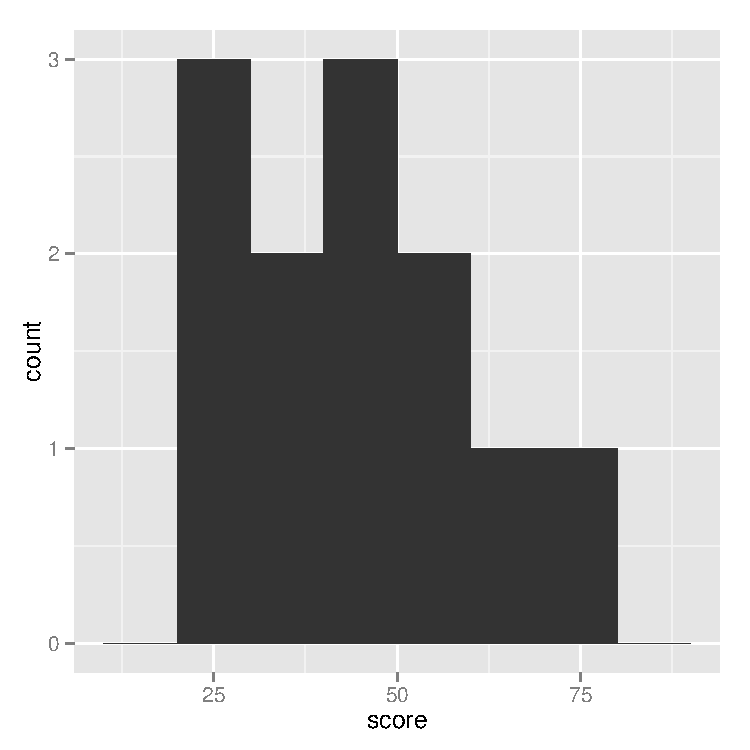
\includegraphics[width=.5\maxwidth]{figure/hsito-1} 

\end{knitrout}
\end{center}

\item For \textbf{both} the Cornhuskers and the Wolverines, calculate the first quartile, the median, and the third quartile using the quartile function $Q(p)$.

\ben
\item 

\item Construct side-by-side boxplots comparing the data for the Wolverines and the Cornhuskers. Make the axis range from 20 to 80 points with tick marks every 10 units. Based on the boxplots, are there \emph{unusual} observations for either school?

\item Construct a quantile-quantile plot to compare the shape of the two distributions. Would you say that the plot appears to be linear? What does that indicate about the shapes of the two distributions? 

\item Construct a theoretical quantile-quantile plot using a normal distribution as the theoretical normal probability plot for the Wolverines.The table below displays the quantiles of the theoretical normal distribution when $n=12$:

\begin{center}
\begin{tabular}{| l | c c c c c c |}\hline
	$p$ & 1/24 & 3/24 & 5/24 & 7/24 & 9/24 & 11/24\\
	$Q(p)$ & -1.73 & -1.15 & -0.81 & -0.55 & -0.32 & -0.10\\ \hline\hline
	$p$ & 13/24 & 15/24 & 17/24 & 19/24 & 21/24 & 23/24\\
	$Q(p)$ & 0.10 & 0.32 & 0.55 & 0.81 & 1.15 & 1.73\\\hline
\end{tabular}
\end{center}

Would you say that the plot appears to be linear? Does this imply the Wolverines football scores could have come from a normal distribution?

\item Calculate the sample mean, sample variance, and sample standard deviation for each school. Clearly label your answers.\\
\emph{Hint: for the Wolverines} $\dsum^{12}_{i=1} x_i = 322$, $\dsum^{12}_{i=1} x_i^2 = 9074$, \\ \emph{and for the Cornhuskers} $\dsum^{12}_{i=1} x_i = 548$, $\dsum^{12}_{i=1} x_i^2 = 27900$.


\een

\pagebreak

\item 
   The NBA uses a salary cap in the hopes to keep the league competitive - the amount each team can spend on player salaries is limited so that no team can acquire all the best players. While this sounds simple in concept, the execution is often complicated and statistical evaluation of players' pay is a popular topic in sports journalism.
   
   The ten highest paying contracts in the 2015-2016 season are:
%-- Name: R code (Code in Document)
\begin{kframe}


{\ttfamily\noindent\itshape\color{messagecolor}{\#\# \\\#\# Attaching package: 'dplyr'\\\#\# \\\#\# The following object is masked from 'package:stats':\\\#\# \\\#\#\ \ \ \  filter\\\#\# \\\#\# The following objects are masked from 'package:base':\\\#\# \\\#\#\ \ \ \  intersect, setdiff, setequal, union}}\end{kframe}% latex table generated in R 3.1.3 by xtable 1.7-4 package
% Thu Sep 17 15:06:19 2015
\begin{table}[ht]
\centering
\begin{tabular}{rllr}
  \hline
 & player & team & salary2015 \\ 
  \hline
1 & Kobe Bryant & LAL & 25000000 \\ 
  2 & Joe Johnson & BRK & 24894863 \\ 
  3 & LeBron James & CLE & 22971000 \\ 
  4 & Carmelo Anthony & NYK & 22875000 \\ 
  5 & Dwight Howard & HOU & 22359364 \\ 
  6 & Chris Bosh & MIA & 22192730 \\ 
  7 & Chris Paul & LAC & 21468696 \\ 
  8 & Kevin Durant & OKC & 20158622 \\ 
  9 & Derrick Rose & CHI & 20093063 \\ 
  10 & Brook Lopez & BRK & 20000000 \\ 
   \hline
\end{tabular}
\end{table}



   
   Below are three histogram's summarizing the salary of each player. \\

%-- Name: R code (Code in Document)
\begin{knitrout}
\definecolor{shadecolor}{rgb}{0.969, 0.969, 0.969}\color{fgcolor}
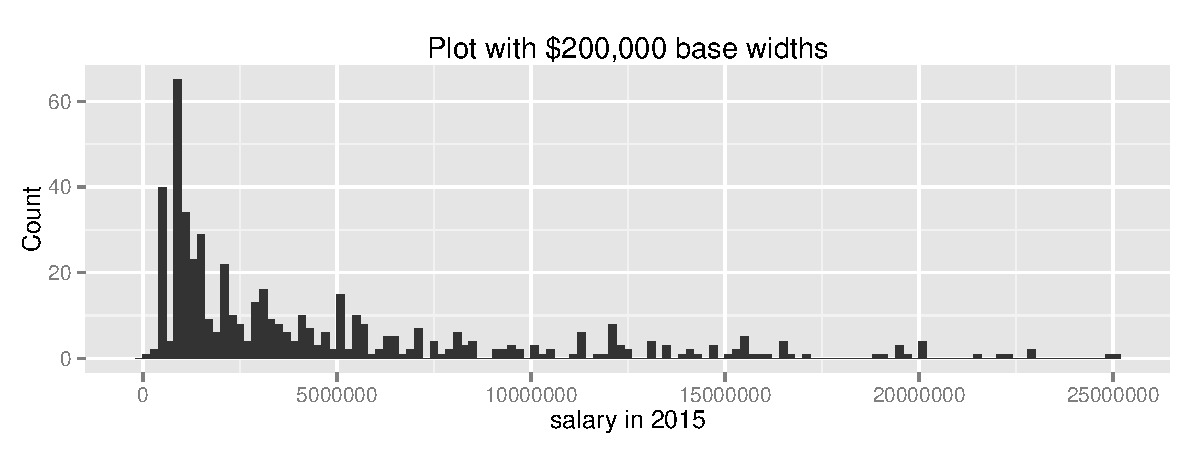
\includegraphics[width=\maxwidth]{figure/unnamed-chunk-2-1} 

\end{knitrout}

%-- Name: R code (Code in Document)
\begin{knitrout}
\definecolor{shadecolor}{rgb}{0.969, 0.969, 0.969}\color{fgcolor}
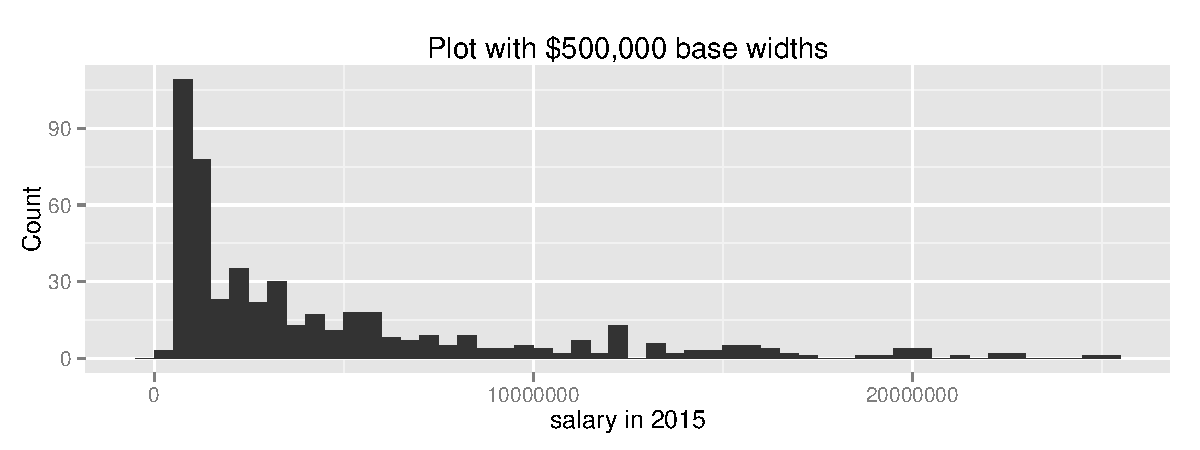
\includegraphics[width=\maxwidth]{figure/unnamed-chunk-3-1} 

\end{knitrout}

Note that the width of the intervals is the only important feature thing that changes between the two plots

\ben
   \item Which of the two histograms do you thing does a better job of summarizing the data (meaning which plot helps you get a better picture of what is happening with salaries in the NBA)?
   \item Using the terminalogy from class and discussed in section 3.1.2, describe the distribution of yards per game. Be sure to comment on the number of modes and symmetry.
	\item Does the sample mean or sample median provide a more appropriate measure of center (location) of the distribution of 2015 NBA salaries? Explain briefly.
	\item Does the sample standard deviation or sample IQR provide a more appropriate measure of spread (variability) of the distribution of 2015 NBA salaries? Explain briefly.

There is also information on the anticipated salary for players next season who are under contract at that point. Here are the top ten salaries for next year's players:
%-- Name: R code (Code in Document)
% latex table generated in R 3.1.3 by xtable 1.7-4 package
% Thu Sep 17 15:06:20 2015
\begin{table}[ht]
\centering
\begin{tabular}{rllr}
  \hline
 & player & team & salary2016 \\ 
  \hline
1 & Carmelo Anthony & NYK & 24559380 \\ 
  2 & LeBron James & CLE & 24004000 \\ 
  3 & Chris Bosh & MIA & 23741060 \\ 
  4 & Dwight Howard & HOU & 23282457 \\ 
  5 & Chris Paul & LAC & 22868828 \\ 
  6 & Kevin Love & CLE & 21500000 \\ 
  7 & DeAndre Jordan & LAC & 21500000 \\ 
  8 & Derrick Rose & CHI & 21323250 \\ 
  9 & Marc Gasol & MEM & 21200000 \\ 
  10 & Damian Lillard & POR & 21000000 \\ 
   \hline
\end{tabular}
\end{table}

We can create a scatter plot of the current salary and next seasons salary:

%-- Name: R code (Code in Document)
\begin{knitrout}
\definecolor{shadecolor}{rgb}{0.969, 0.969, 0.969}\color{fgcolor}
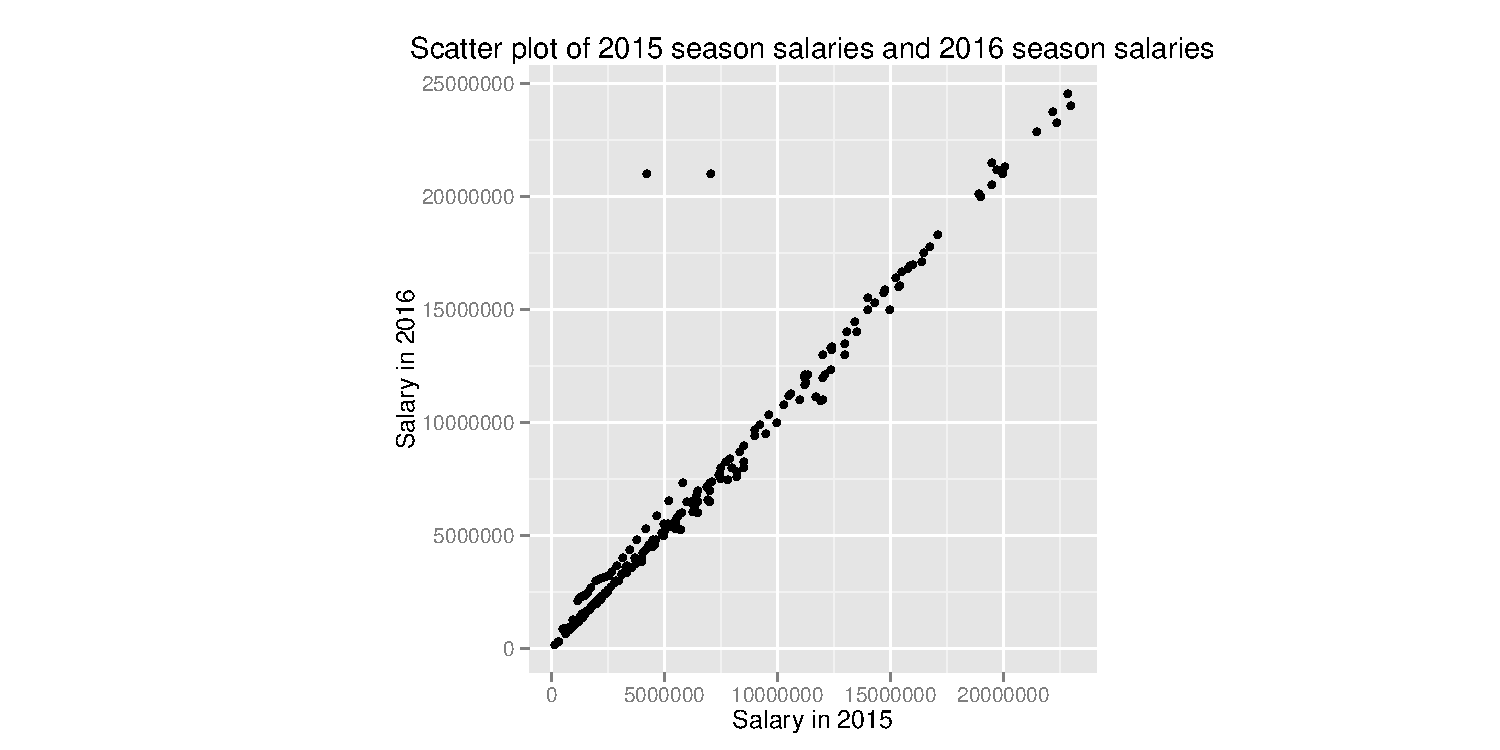
\includegraphics[width=\maxwidth]{figure/unnamed-chunk-5-1} 

\end{knitrout}

We can also look at each team's salary information: 

\begin{knitrout}
\definecolor{shadecolor}{rgb}{0.969, 0.969, 0.969}\color{fgcolor}
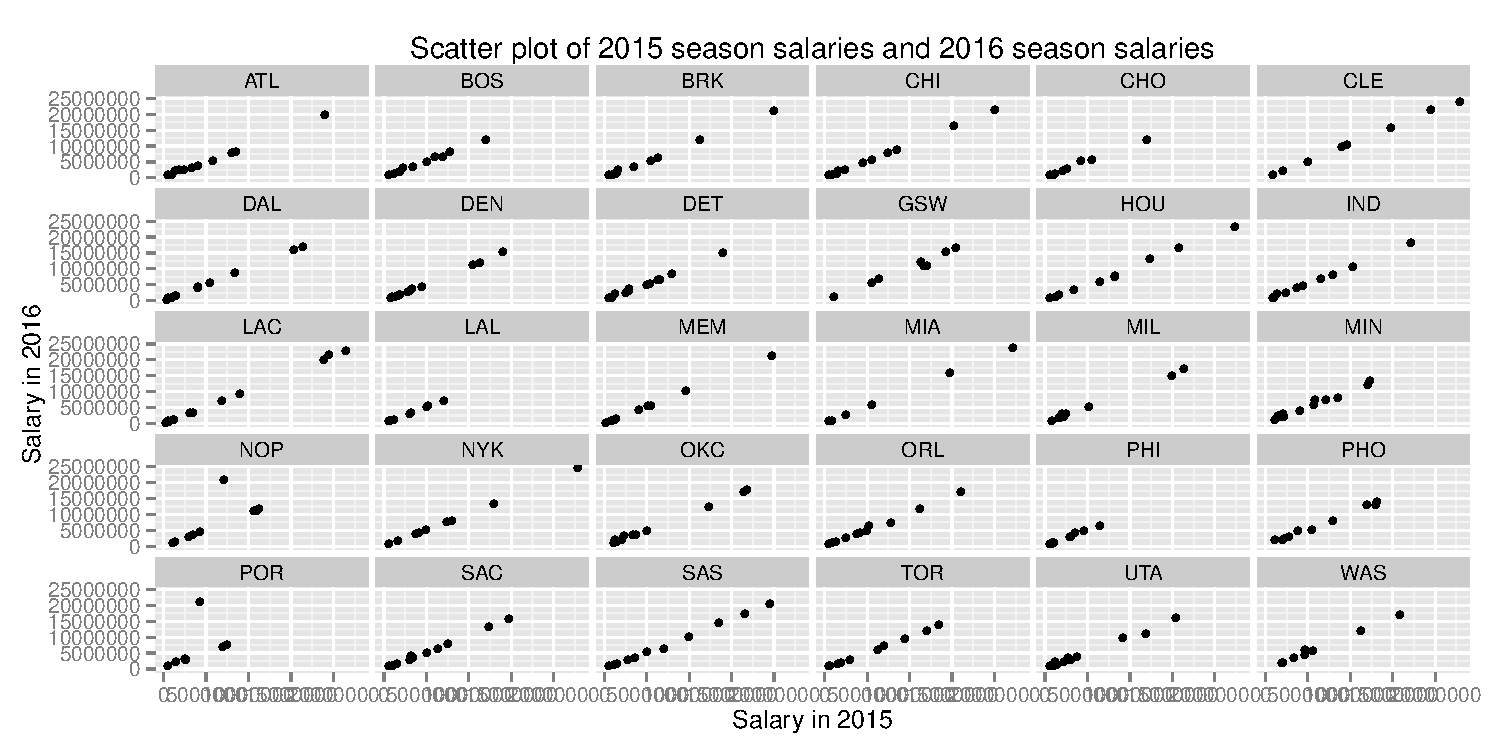
\includegraphics[width=\maxwidth]{figure/unnamed-chunk-6-1} 

\end{knitrout}

   \item Describe the relationship between the 2015 season salary and the 2016 season salary.
   \item What sort of structural features/curiosities are present in this data set? Explain.
\een


\clearpage

\item \textbf{JMP Assignment.} 

   Without laboring the point, computing is one of the most important parts of modern data analysis. A large part of data science simply wouldn't exist without the tools developed by scientists working at the intersections of computer science, mathematics, and statistics. 
   Because of that, there will inevitably be parts of this course where a statistical computing tools are needed. SAS and R are the two main languages used by statisticians, with Python, Julia, F\#, C++ and others making important contributions as well.
   SAS has a software called JMP ("Jump") that makes doing statistical analyses simpler - it is more powerful than Excel or your calculator but requires little in the sense of coding making the learning curve much lower. 
   We will be using it this semester. There are labs in Snedecor Hall with the software pre-installed, but it is free for students and I encourage you to download a copy for yourself using the link below.

   Download: \href{http://www.stat.iastate.edu/resources-2/software-sasjmpr/statistical-software-jmp/}{http://www.stat.iastate.edu/resources-2/software-sasjmpr/statistical-software-jmp/}

   Additionally, you may want to consider the following tutorials (they are very helpful):
   
   Tutorials: \href{http://web.utk.edu/~cwiek/201Tutorials/}{http://web.utk.edu/~cwiek/201Tutorials/} 

   The tutorials cover the following topics:
   \begin{itemize}
     \item Histogram and Box Plot
     \item Stem and Leaf Plot
     \item Normal Probability Plot and Goodness of Fit Test
     \item Calculating Summary Statistics of Quantitative Data
     \item Getting JMP Graphics into Microsoft Word
   \end{itemize}

   For this problem I am asking you to:

   \begin{enumerate}
      \item Download and install \texttt{JMP} or find a computer with it already installed.
      \item Take a screen shot once you have it open.
   \end{enumerate}

\een


\end{document}
